\documentclass[12pt,a4paper]{report}
\usepackage[utf8]{inputenc}
\usepackage{amsmath}
\usepackage{amsfonts}
\usepackage{amssymb}
\usepackage{graphicx}
\usepackage{geometry}
\usepackage{float}
\usepackage{caption}
\usepackage{subcaption}
\usepackage{booktabs}
\usepackage{hyperref}
\usepackage{xcolor}

\geometry{margin=1in}
\hypersetup{
    colorlinks=true,
    linkcolor=blue,
    filecolor=magenta,      
    urlcolor=cyan,
}

\title{\textbf{MSDS 7333 - Final Case Study \\ Financial Loss Minimization \\ through Binary Classification}}
\author{Tue Vu}
\date{\today}

\begin{document}

\maketitle

\newpage

\chapter{Introduction}

This is the final case study for the MSDS 7333 course. 
The given data is a structured dataset \textbf{final\_project.csv} that contains 160,000 observations with 51 features, representing a substantial but manageable dataset for machine learning applications.
The objective of this study is to develop a predictive model that minimizes financial losses in a production environment. The business problem is characterized by significant monetary penalties associated with misclassification:

\begin{itemize}
    \item \textbf{False Positive Cost}: When we predict class 1 but the true class is 0, we incur a loss of \$100
    \item \textbf{False Negative Cost}: When we predict class 0 but the true class is 1, we incur a loss of \$100
\end{itemize}

The equal cost structure for both types of misclassification makes this a balanced cost-sensitive classification problem. The goal is to minimize the total financial loss rather than simply maximizing accuracy, which requires careful consideration of the prediction threshold and model performance metrics.

This study employs a systematic supervised binary classification machine learning approach.
The data size is substantial for tree-based models, but not too large for neural network models. Therefore, XGBoost is chosen as the primary modeling algorithm.
The content of this report is organized as follows:
\begin{itemize}
    \item \textbf{Chapter 1: Data Overview}: Overview of the dataset and report objectives
    \item \textbf{Chapter 2: Exploratory Data Analysis}: Introduce about the data, methodology used in this report and Exploratory data analysis of the dataset
    \item \textbf{Chapter 3: Modeling}: Supervised ML Classification of the dataset using XGBoost
    \item \textbf{Chapter 4: Discussion and Conclusions}: Discussions and conclusions of the study
\end{itemize}

\chapter{Exploratory Data Analysis}

The dataset consists of 160,000 observations with 51 features (x0 to x49) plus 1 target variable (y), representing a substantial but manageable dataset for machine learning applications. 
Within the 50 input features, there are 45 numerical features and 5 categorical features (x24, x29, x30, x32, x37).
The target variable is binary classification (0, 1).

Based on a quick look at the data, the categorical features appear to represent Geographic regions (Asia, Europe, America) in \textbf{x24}, Temporal patterns (months, with summer concentration) in \textbf{x29}, Day-of-week patterns (weekday focus) in \textbf{x30}, Percentage values (0.0\% to 0.05\% range) in \textbf{x32}, and Currency amounts (converted from string format) in \textbf{x37}.
The data appears to represent cross-continental travel incidents, with seasonal and geographic patterns that may be relevant for prediction.
The dataset demonstrates high data quality with minimal missing values across all features. Figure \ref{fig:missing_values} shows the distribution of missing values, with the highest percentage being only 0.03\% for feature x23.

From Figure \ref{fig:missing_values}, we can see that the missing values are minor and distributed across almost all features, with the highest percentage being only 0.03\% for feature x23.
The target variable (y) has no missing values.
In overall, the data is complete and suitable for imputation rather than deletion.
To impute the missing values, with the understanding that the missing data is not too large and the data is related to temporal patterns such as weekday, month, and year.
Therefore, KNN imputation is used for numerical features with the advantage of preserving the nearest neighbor relationship with the other data points.
For categorical features, the most frequent value is used to impute the missing data.

\begin{figure}[H]
    \centering
    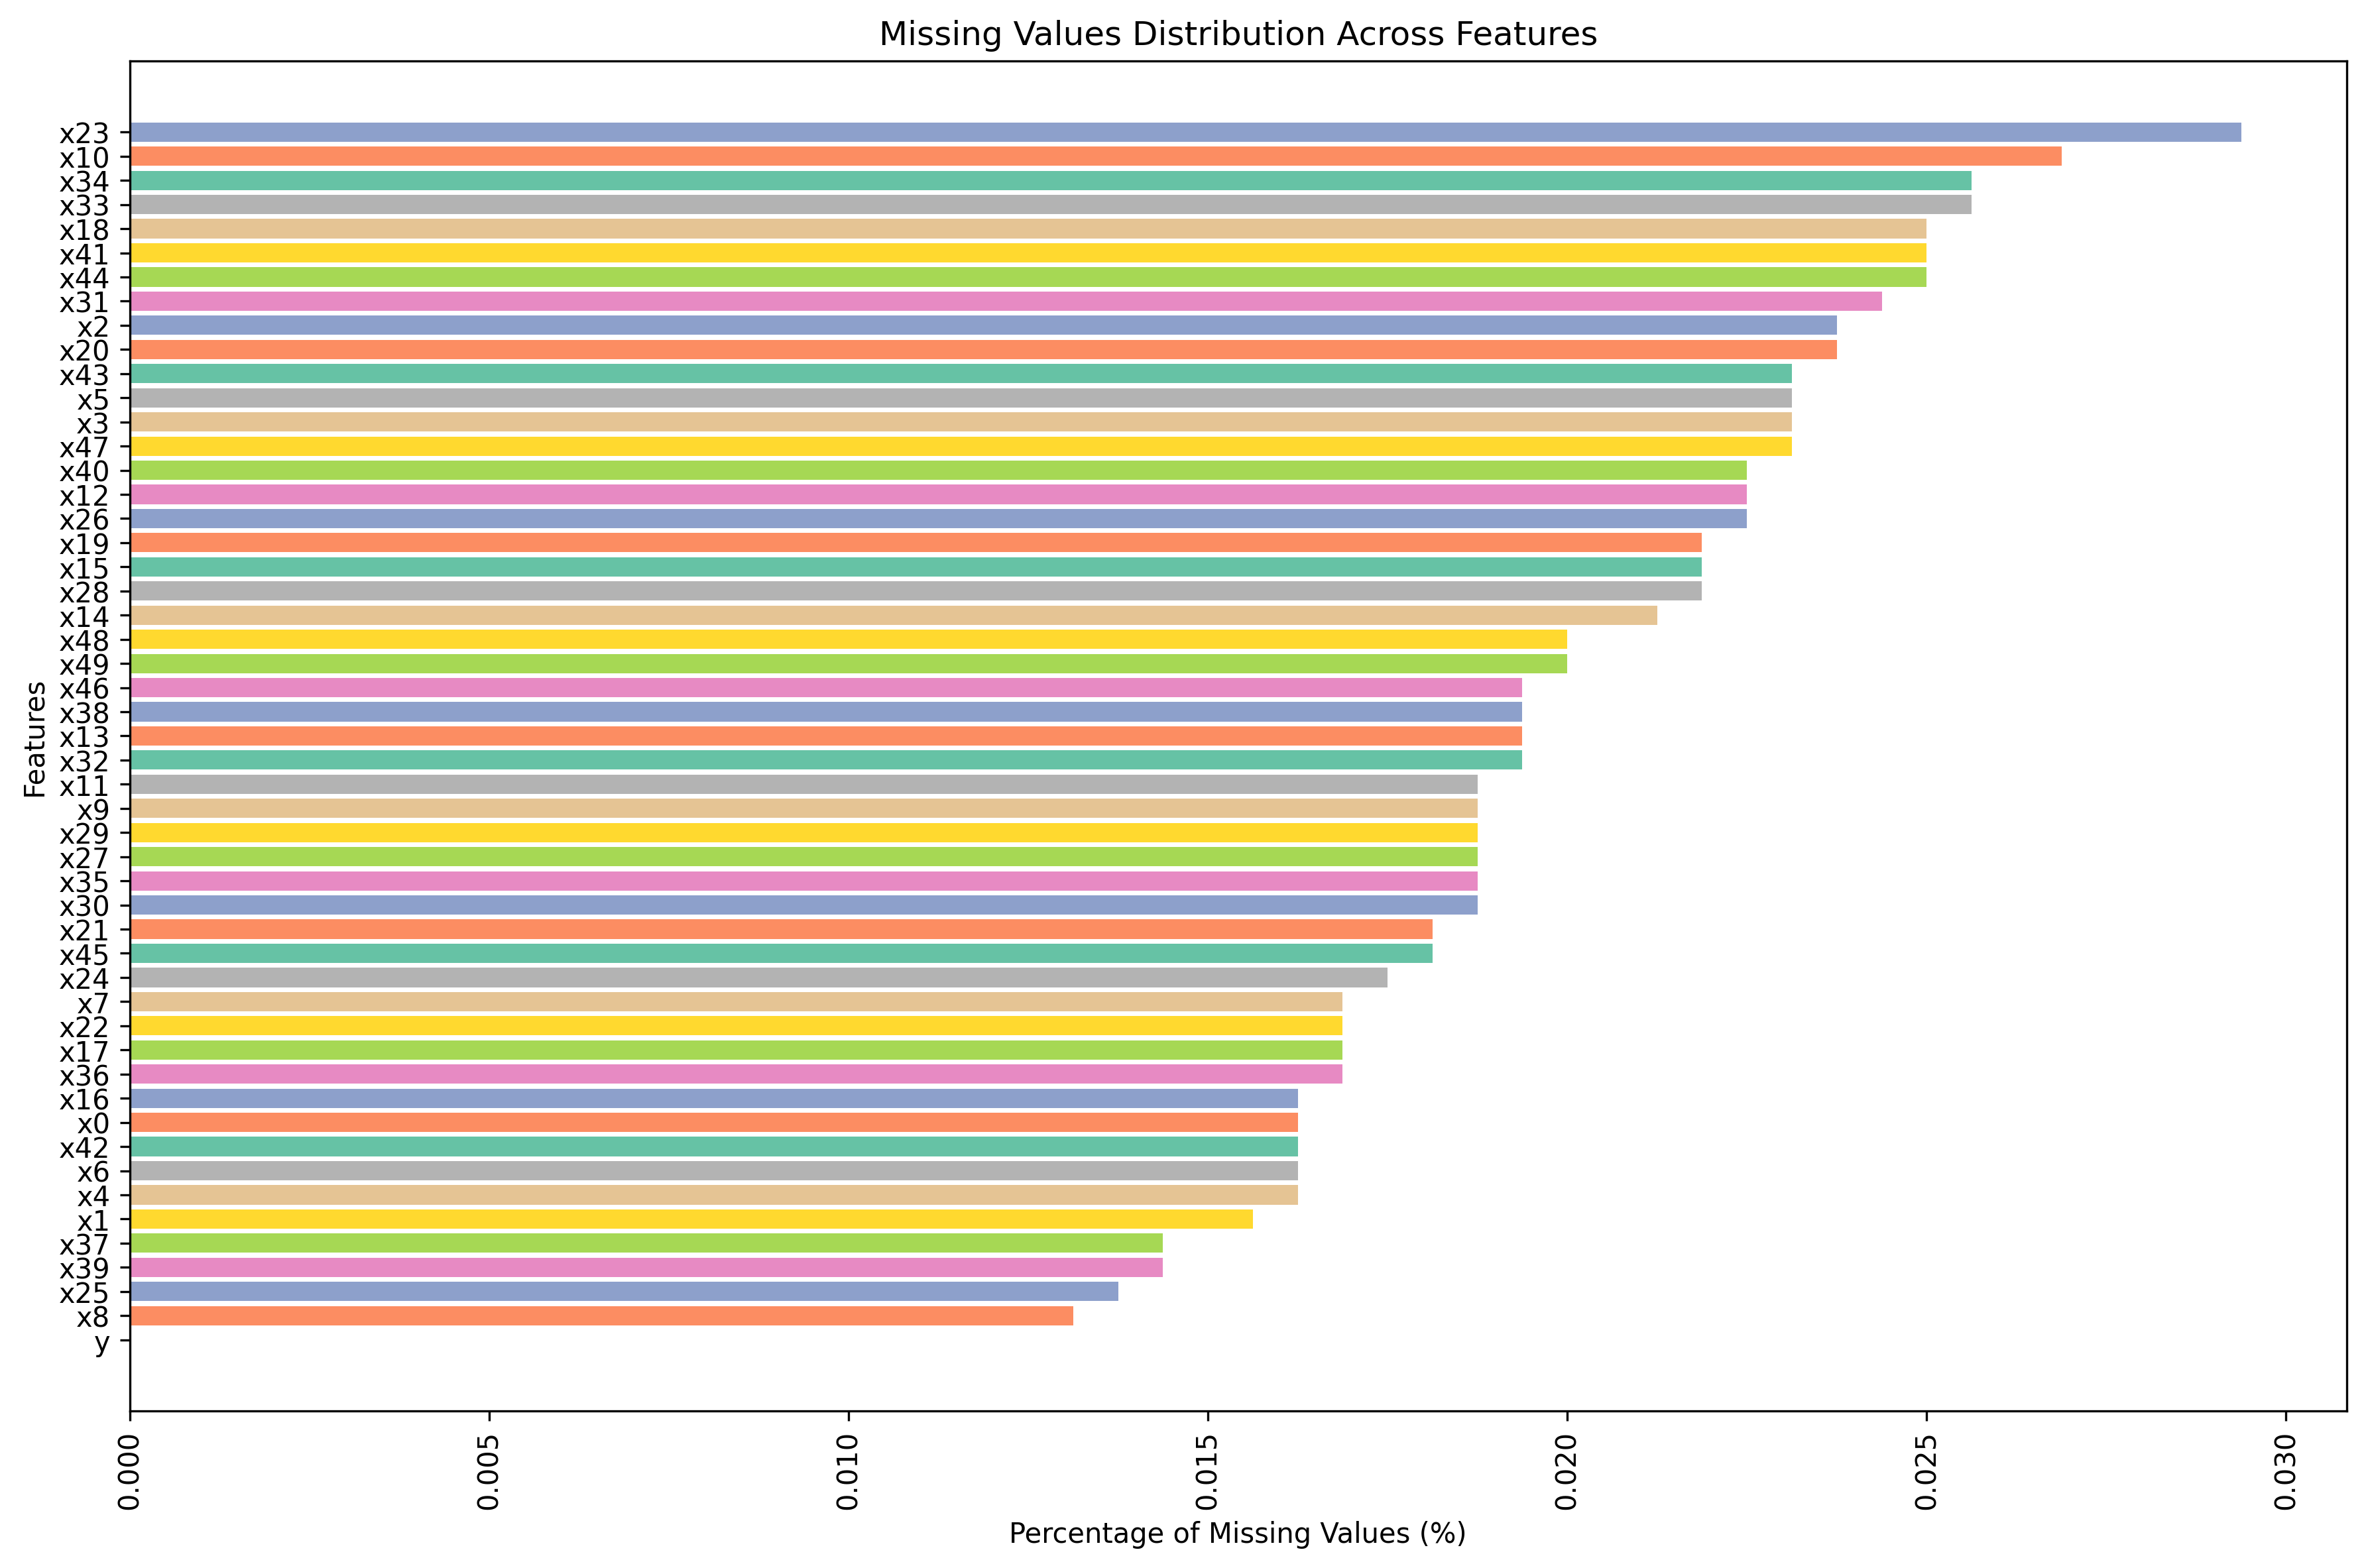
\includegraphics[width=1\textwidth]{plots/missing_values.png}
    \caption{Missing Values Distribution Across Features}
    \label{fig:missing_values}
\end{figure}

From the barplot in Figure \ref{fig:label_count}, the target variable distribution shows a moderately imbalanced dataset with a reasonable split between classes.
The class 1 has 40\% of the observations and class 0 has 60\% of the observations.
This distribution is sufficiently balanced for standard classification techniques without requiring specialized sampling methods.

\begin{figure}[H]
    \centering
    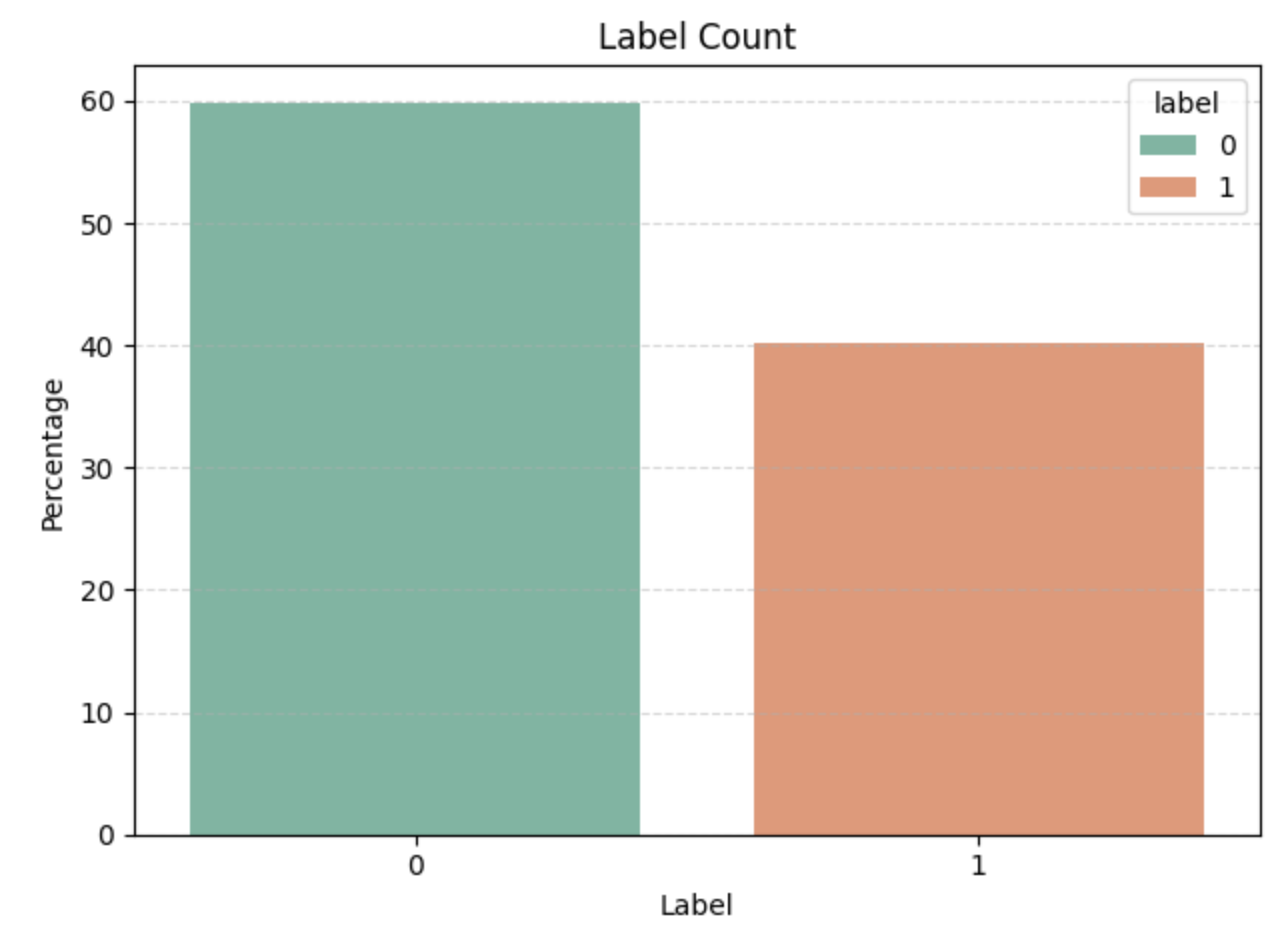
\includegraphics[width=0.6\textwidth]{plots/label_count.png}
    \caption{Distribution of Target Variable Classes}
    \label{fig:label_count}
\end{figure}

The categorical features on the other hand reveal interesting patterns that suggest the data represents travel-related incidents.

The barplot in Figure \ref{fig:cat_grid} shows the feature \textbf{x29} with the monthly temporal patterns of the incidents, the pattern reveals that 85\% of incidents occurred in Asia, 10\% in Europe, and 5\% in America. No incidents occurred in other continents.
The feature \textbf{x29} displays the monthly temporal patterns of the incidents with the summer months (June, July, August) accounted for over 75\% of incidents. This strong seasonal concentration suggests that the incidents are related to travel-related activity.
The day-of-week patterns of the incidents (Monday to Friday only) are exhibited in feature \textbf{x30}: highest incidence is on Wednesday, followed by Tuesday and Thursday and very low on Monday and Friday, which are the beggining and end of the week
This pattern is consistent with business travel patterns, where employees are more likely to travel on weekdays.
Last but not least, the feature \textbf{x32} is a percentage feature that represents the percentage of incidents that occurred in the given month with the highest percentage is 0.05\% and the lowest is 0.0\%.
However, the distribution shows that 0.0\% to 0.1\% are the most frequent value and 0.05\% is the least frequent value.
The feature \textbf{x37} on the other hand is a currency feature that represents the currency of the incident. Since the currency is converted from string format we will convert it back to numeric format and put that into the numerical features.
All these categorical features are to be applied one-hot encoding prior to the modeling in Chapter 3.

\begin{figure}[H]
    \centering
    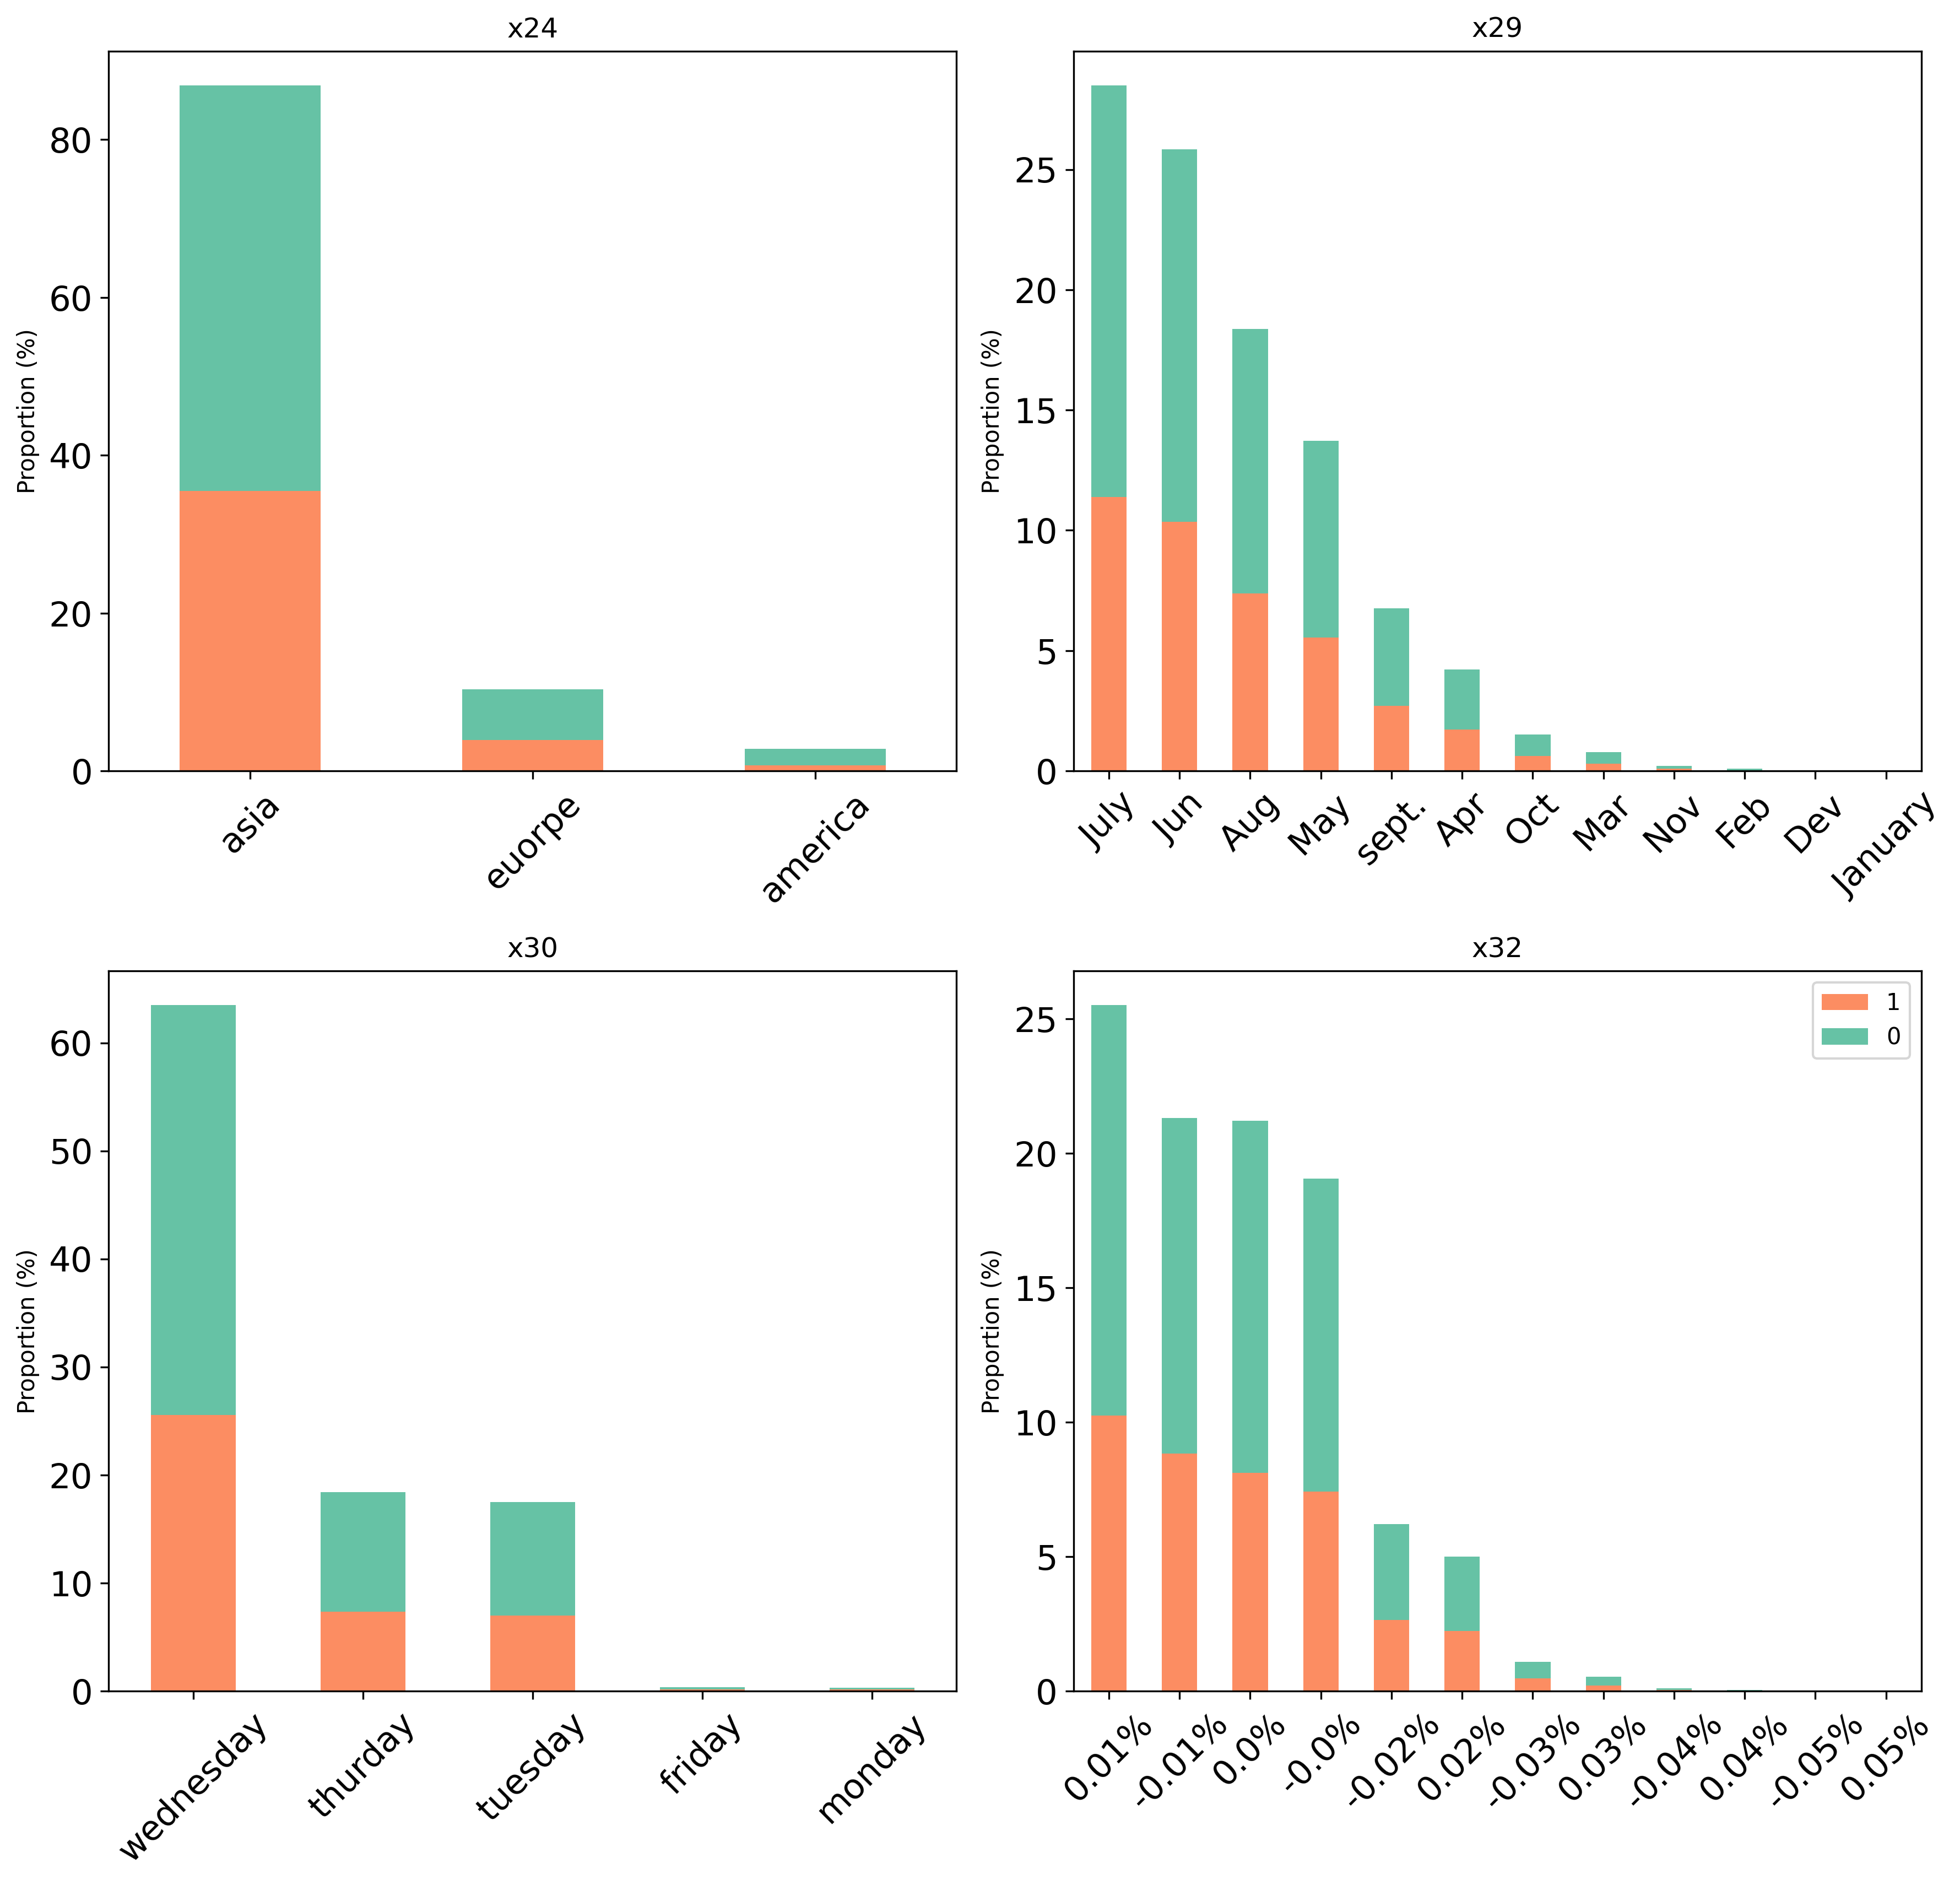
\includegraphics[width=0.9\textwidth]{plots/cat_grid.png}
    \caption{Distribution of Categorical Features by Target Class}
    \label{fig:cat_grid}
\end{figure}

Subsequently, we will perform a cross correlation analysis to identify and remove highly correlated features for numerical features.

\begin{figure}[H]
    \centering
    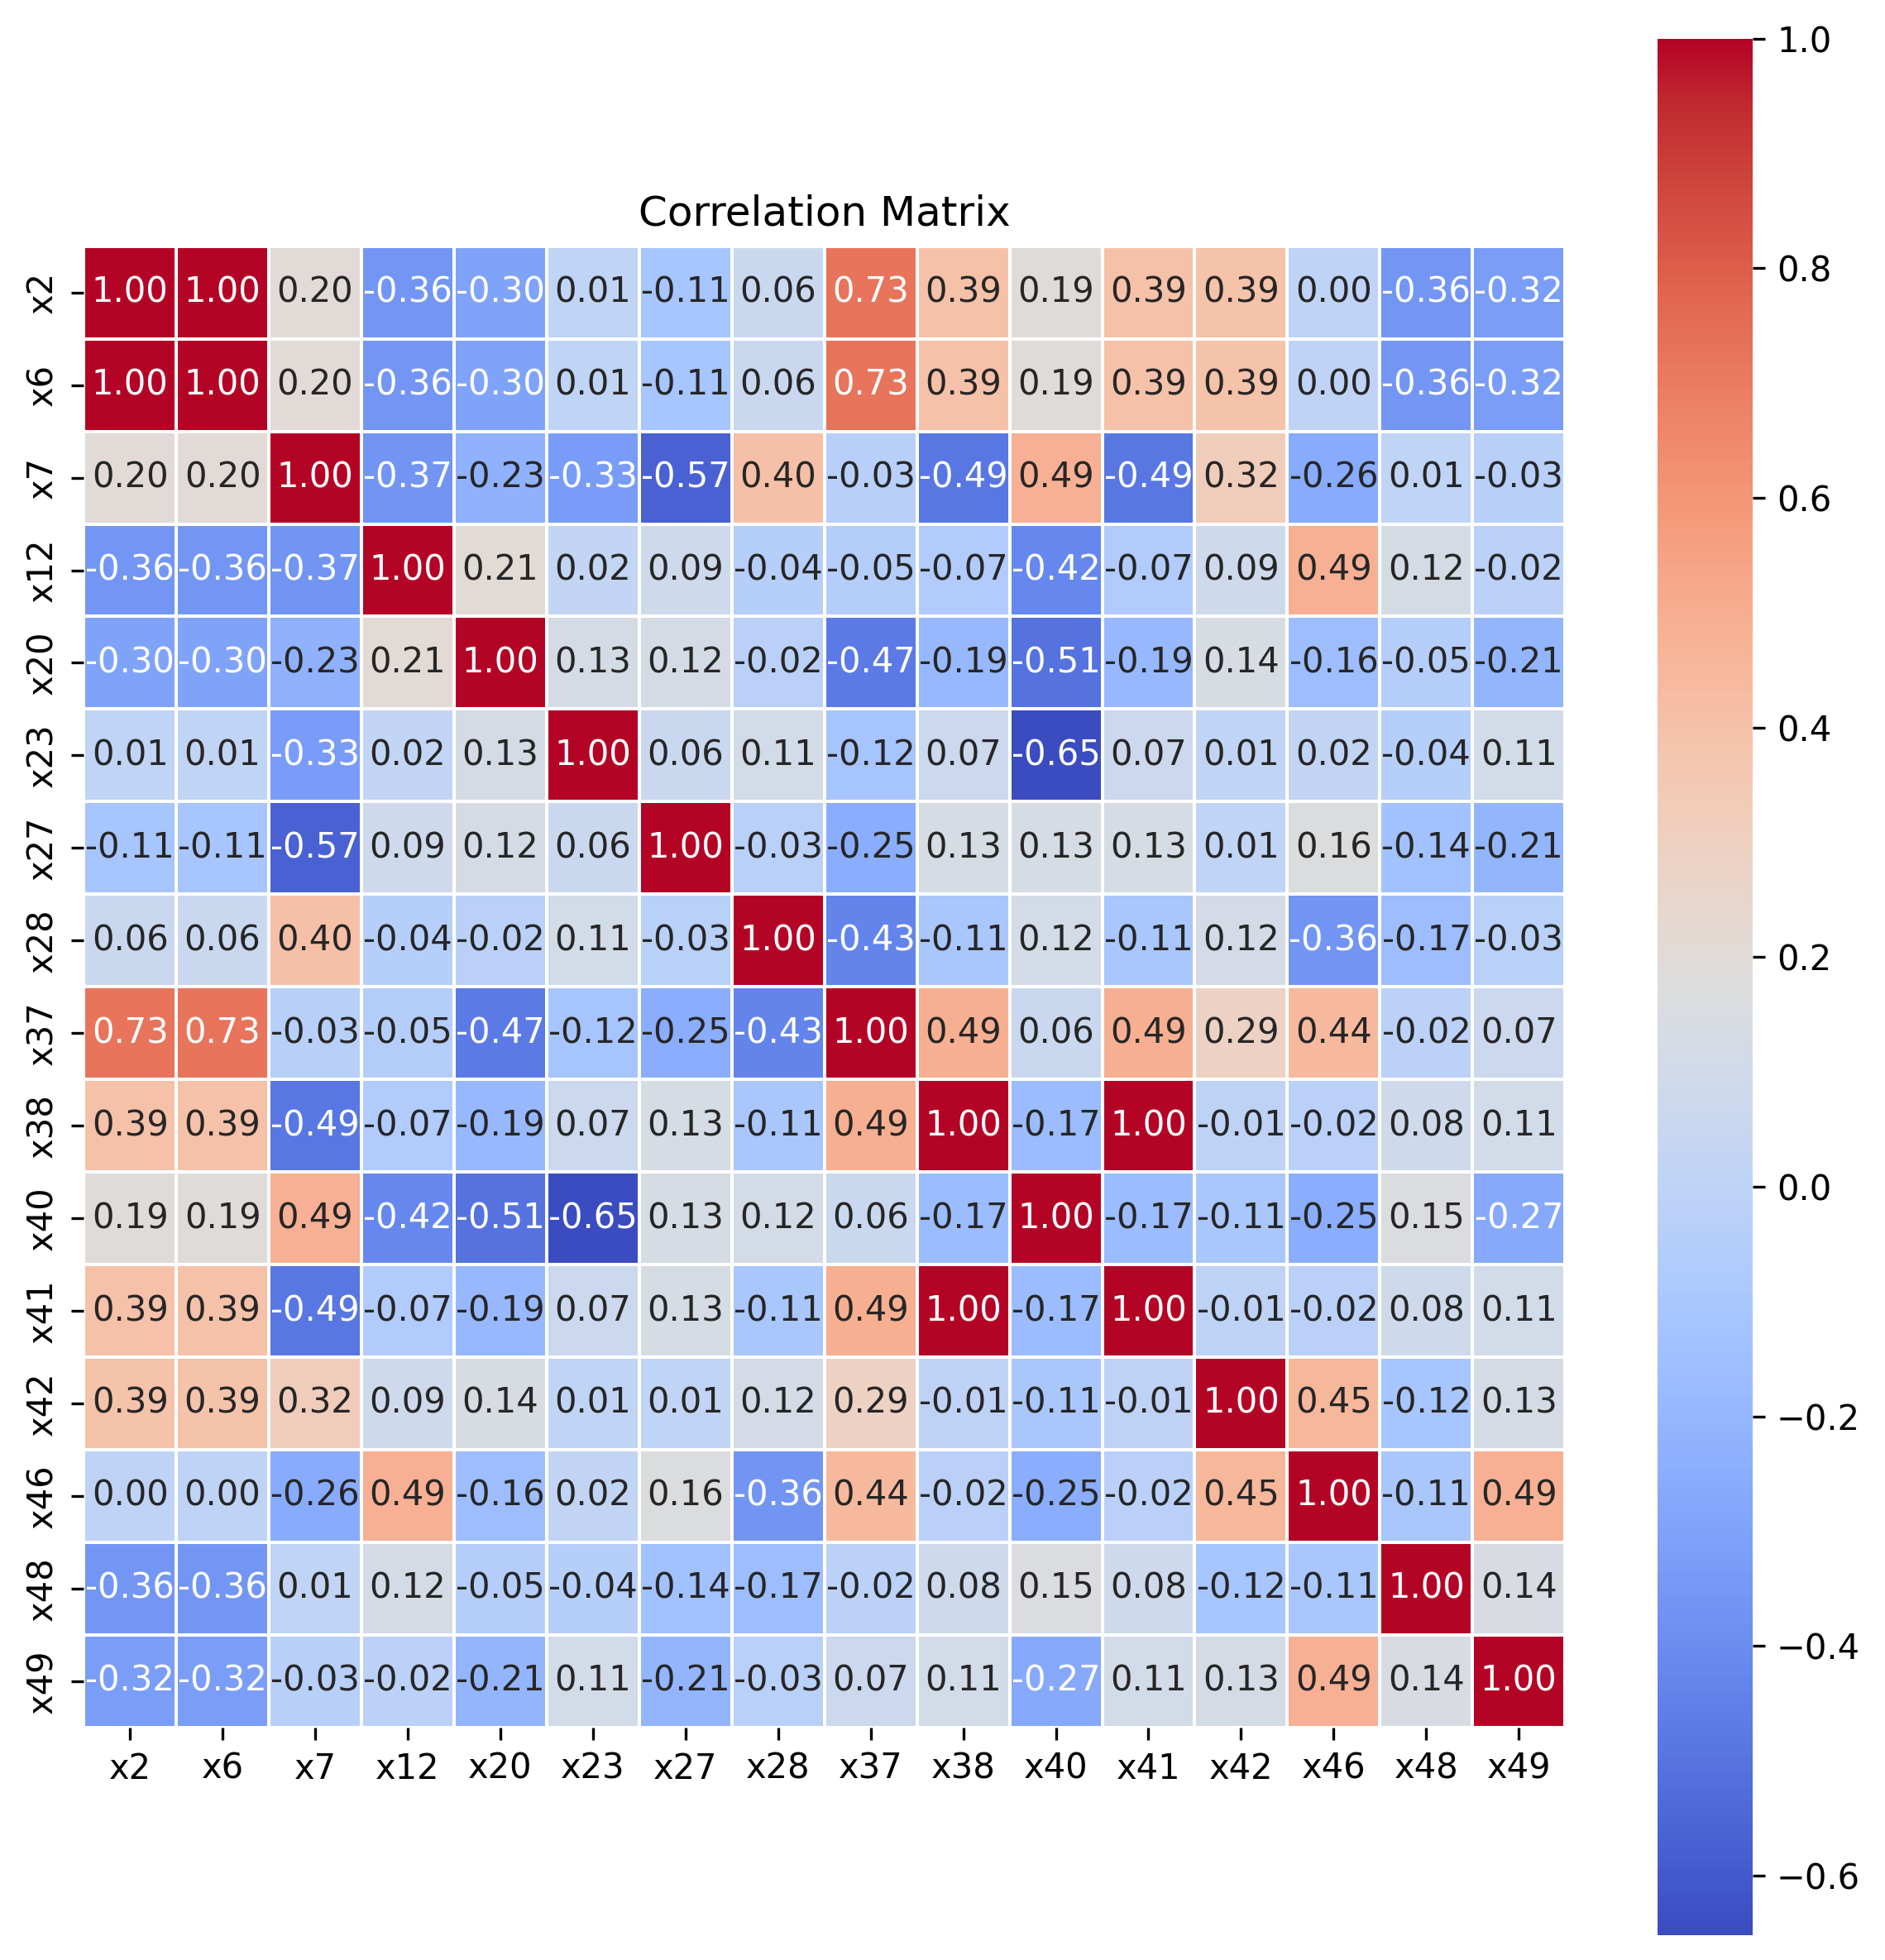
\includegraphics[width=0.8\textwidth]{plots/heatmap.png}
    \caption{Correlation Matrix of High VIF Features}
    \label{fig:heatmap}
\end{figure}

From the heatmap in Figure \ref{fig:heatmap}, we can see that the features pair \textbf{(x2, x6)} and \textbf{(x38, x41)} are highly correlated with a correlation coefficient of 0.99.
It potentially indicates that the features are redundant and should be removed to reduce multicollinearity. We will evaluate the VIF values before the removal process. 
We constructed a Table \ref{tab:vif} to show the VIF values for the features with only VIF values more than 10.

\begin{table}[H]
    \centering
    \caption{Variance Inflation Factor (VIF) values for selected variables}
    \begin{tabular}{|c|r|}
    \hline
    \textbf{Variable} & \textbf{VIF} \\
    \hline
    x2   & 34126.355432 \\
    x6   & 34057.358852 \\
    x7   & 12478.838091 \\
    x12  & 3195.499162  \\
    x20  & 1897.794550  \\
    x23  & 2244.924924  \\
    x27  & 3896.319704  \\
    x28  & 1167.484493  \\
    x37  & 102.599354   \\
    x38  & 18737.463814 \\
    x40  & 6445.197631  \\
    x41  & 16213.243045 \\
    x42  & 4291.551569  \\
    x46  & 8693.217001  \\
    x48  & 765.091576   \\
    x49  & 4119.394015  \\
    \hline
    \end{tabular}
    \label{tab:vif}
\end{table}

From Table \ref{tab:vif}, we can see that the VIF values are very high for the features \textbf{x2, x6, x38, x41}, which is conincide with our previous analyses using the heatmap.
Therefore, we will remove the features x6, x41 to reduce multicollinearity.

The histogram in Figure \ref{fig:hist_num} shows the distribution analysis of numerical features indicating consistent patterns across the dataset.

\begin{figure}[H]
    \centering
    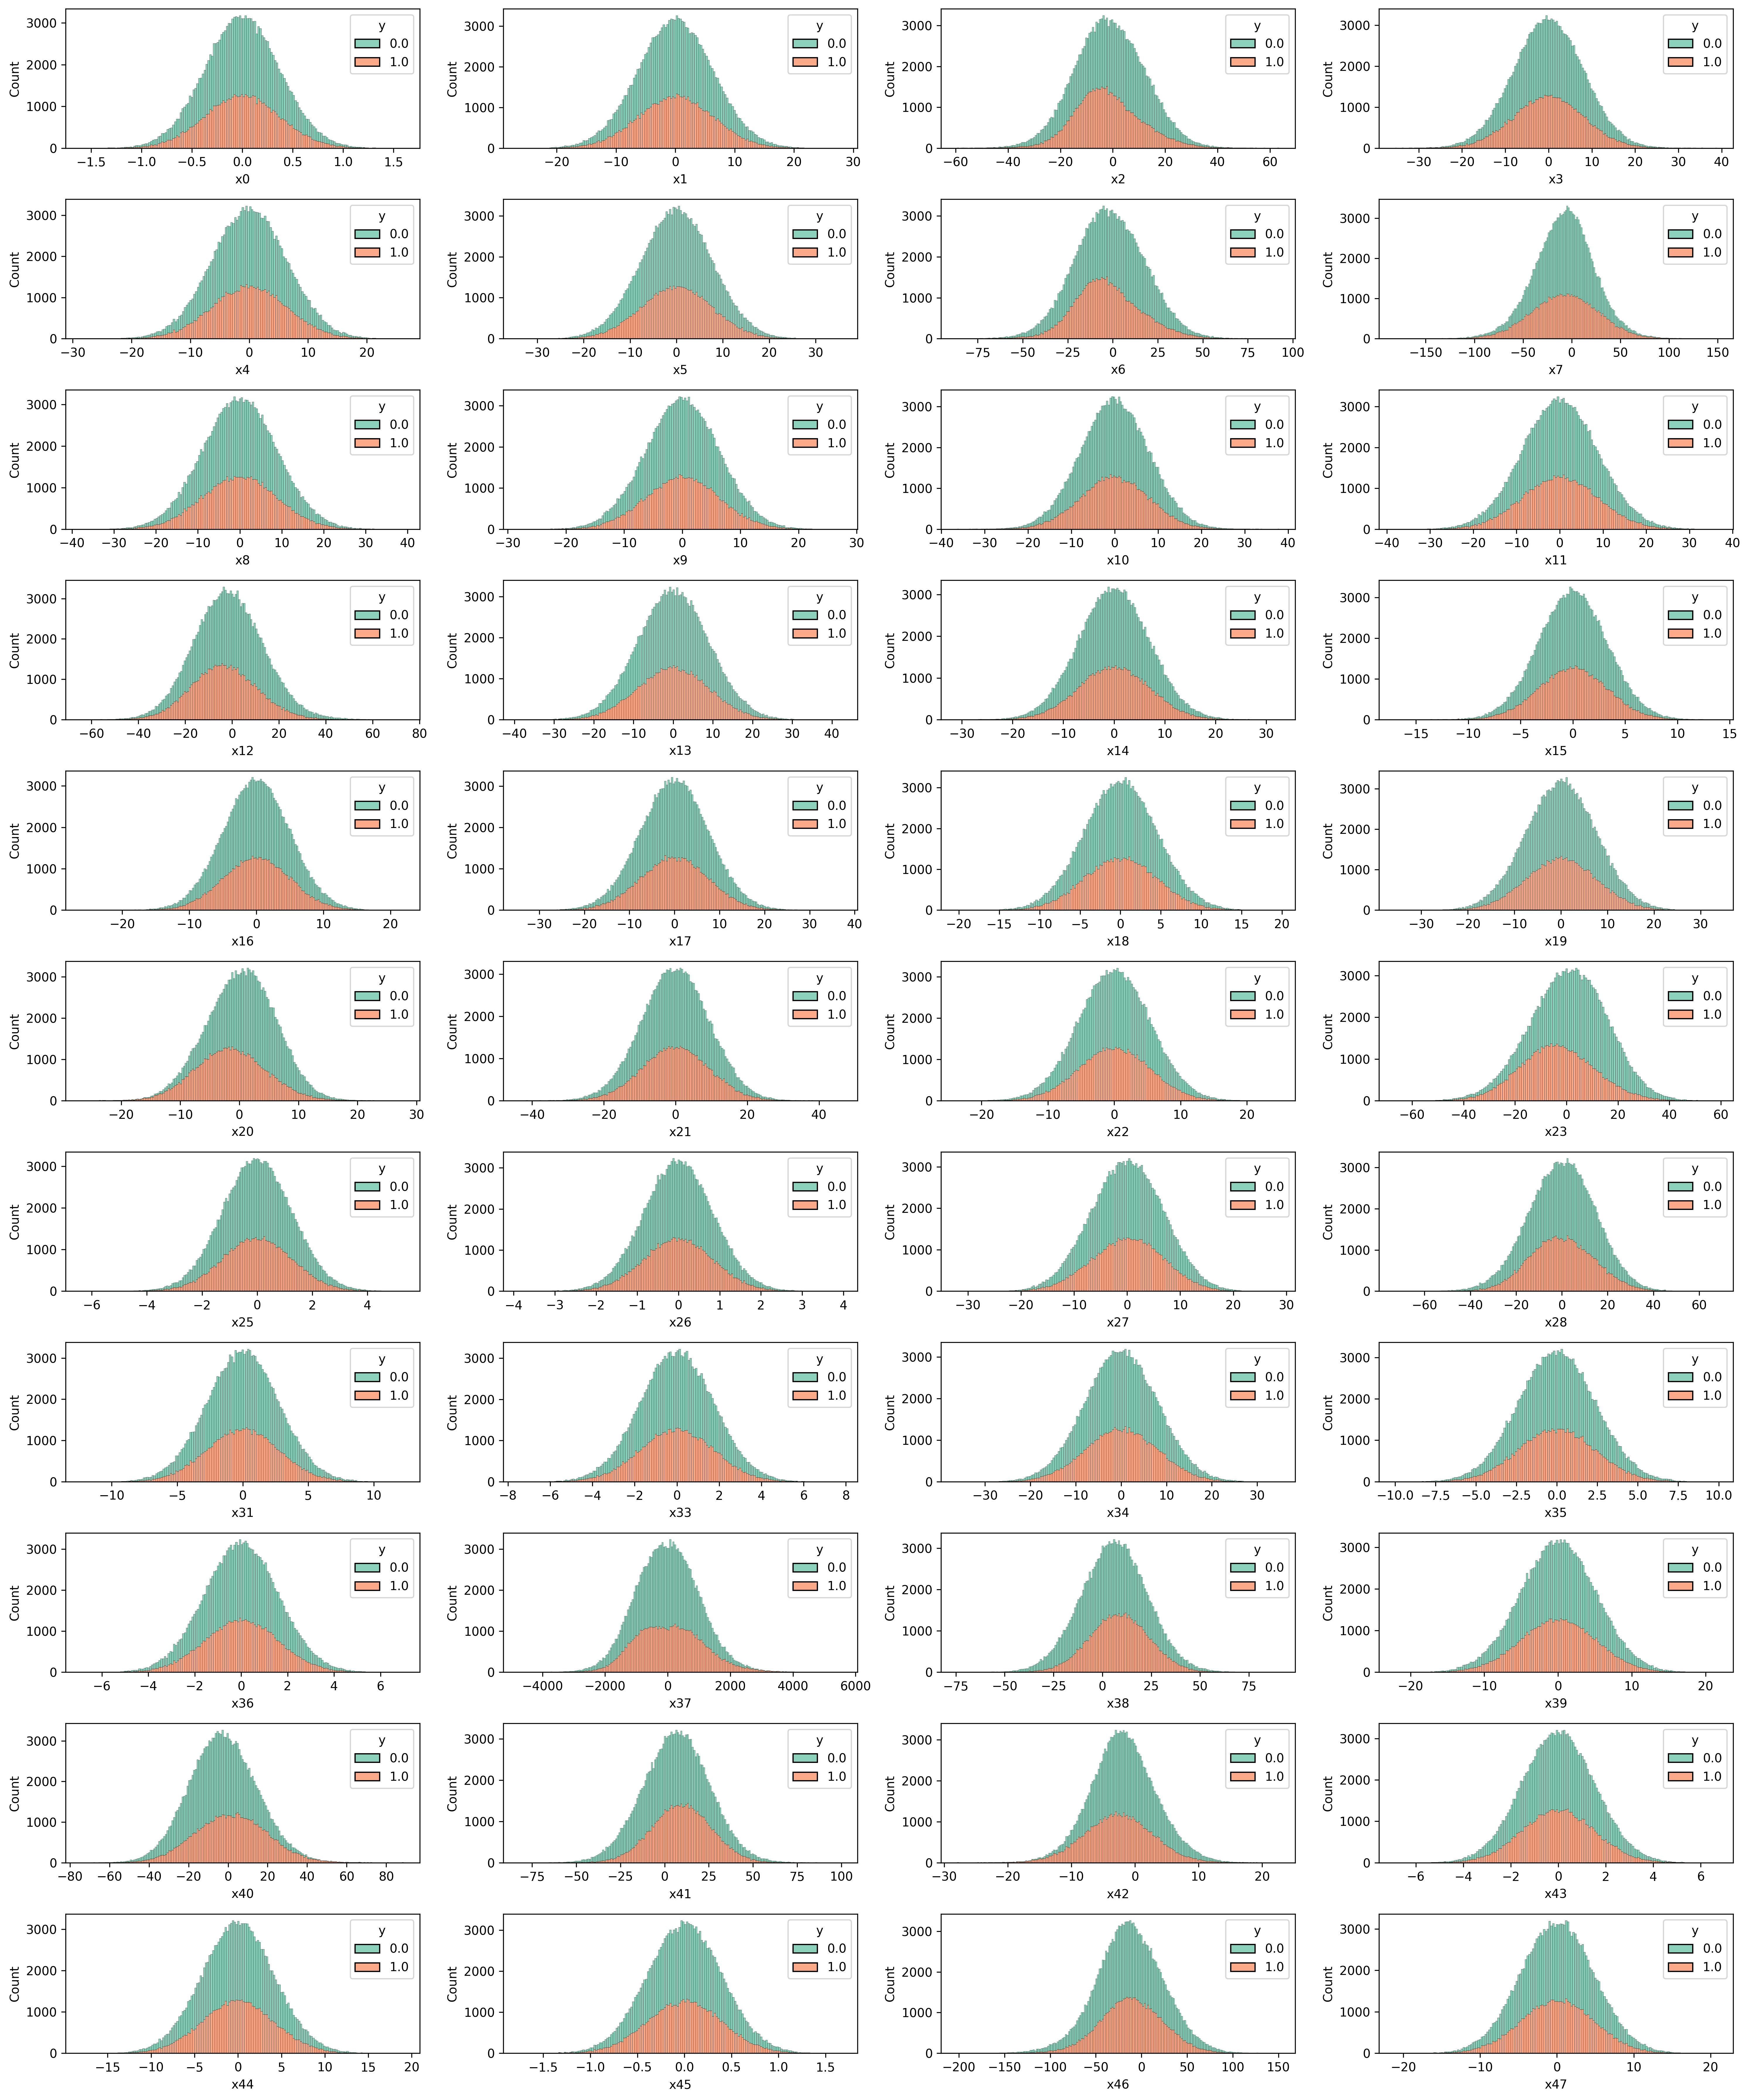
\includegraphics[width=\textwidth]{plots/hist_num.png}
    \caption{Distribution of Numerical Features by Target Class}
    \label{fig:hist_num}
\end{figure}

Figure \ref{fig:hist_num} shows the Gaussian distribution of all the numerical features with bell-shaped curves with varying scales.
No significant skewness is observed, which is suitable for tree-based models without scaling requirements.


\chapter{Modeling}

In this report, the data size with 160,000 observations is too large for Logisgic Regression, Naive Bayes, Random Forest or Support Vector Machine. The training time for these models is too long for CPU training and the model performance degrade due to large dataset.
In addition, the data size is considered small for Neural Network models with many hidden layers. It is well known that for such small dataset the Deep Learning models are not as good as traditional Machine Learning model.
Therefore, we selected XGBoost (Extreme Gradient Boosting) as the primary modeling algorithm based because it is simply one of the best single ML model for supervised learning.
This versaltile tree-based approach does not require to scale the numerical feature and it has excellent performance with mixed data types (numerical and categorical).
The boosting feature enable the ensembling method from growing multiple trees and its built-in regularization help to prevent avoid overfitting.
Lastly, it has the ability to utilize cuda library for acceleration.

The XGBoost model underwent parameter optimization to achieve optimal performance. The final configuration used the following parameters:

\begin{verbatim}
params = {
    'objective': 'binary:logistic', # Binary classification
    'eval_metric': 'logloss',       # Log loss for optimization, with the main objective to reduce the loss
    'learning_rate': 0.1,           # Conservative learning rate
    'max_depth': 20,                # Moderate tree depth
    'subsample': 0.8,               # Prevent overfitting
    'device': 'cuda'                # GPU acceleration
}
\end{verbatim}

The data is split into training and testing sets with 80\% for training and 20\% for testing.
The training data underwent 10-fold cross-validation with 100 \texttt{num\_boost\_round} each to ensure robust performance estimates. 
The cross-validation results are shown in Figure \ref{fig:xgbcv} with the final training AUC is 0.9999 and the final validation AUC is 0.9789. The curves plateau after 60 \texttt{num\_boost\_round}.
The corresponding training log loss is converged to 0.052 and the test log loss is converged to 0.178.
The early stopping of 5 repetition is implemented to prevent overfitting.

\begin{figure}[H]
    \centering
    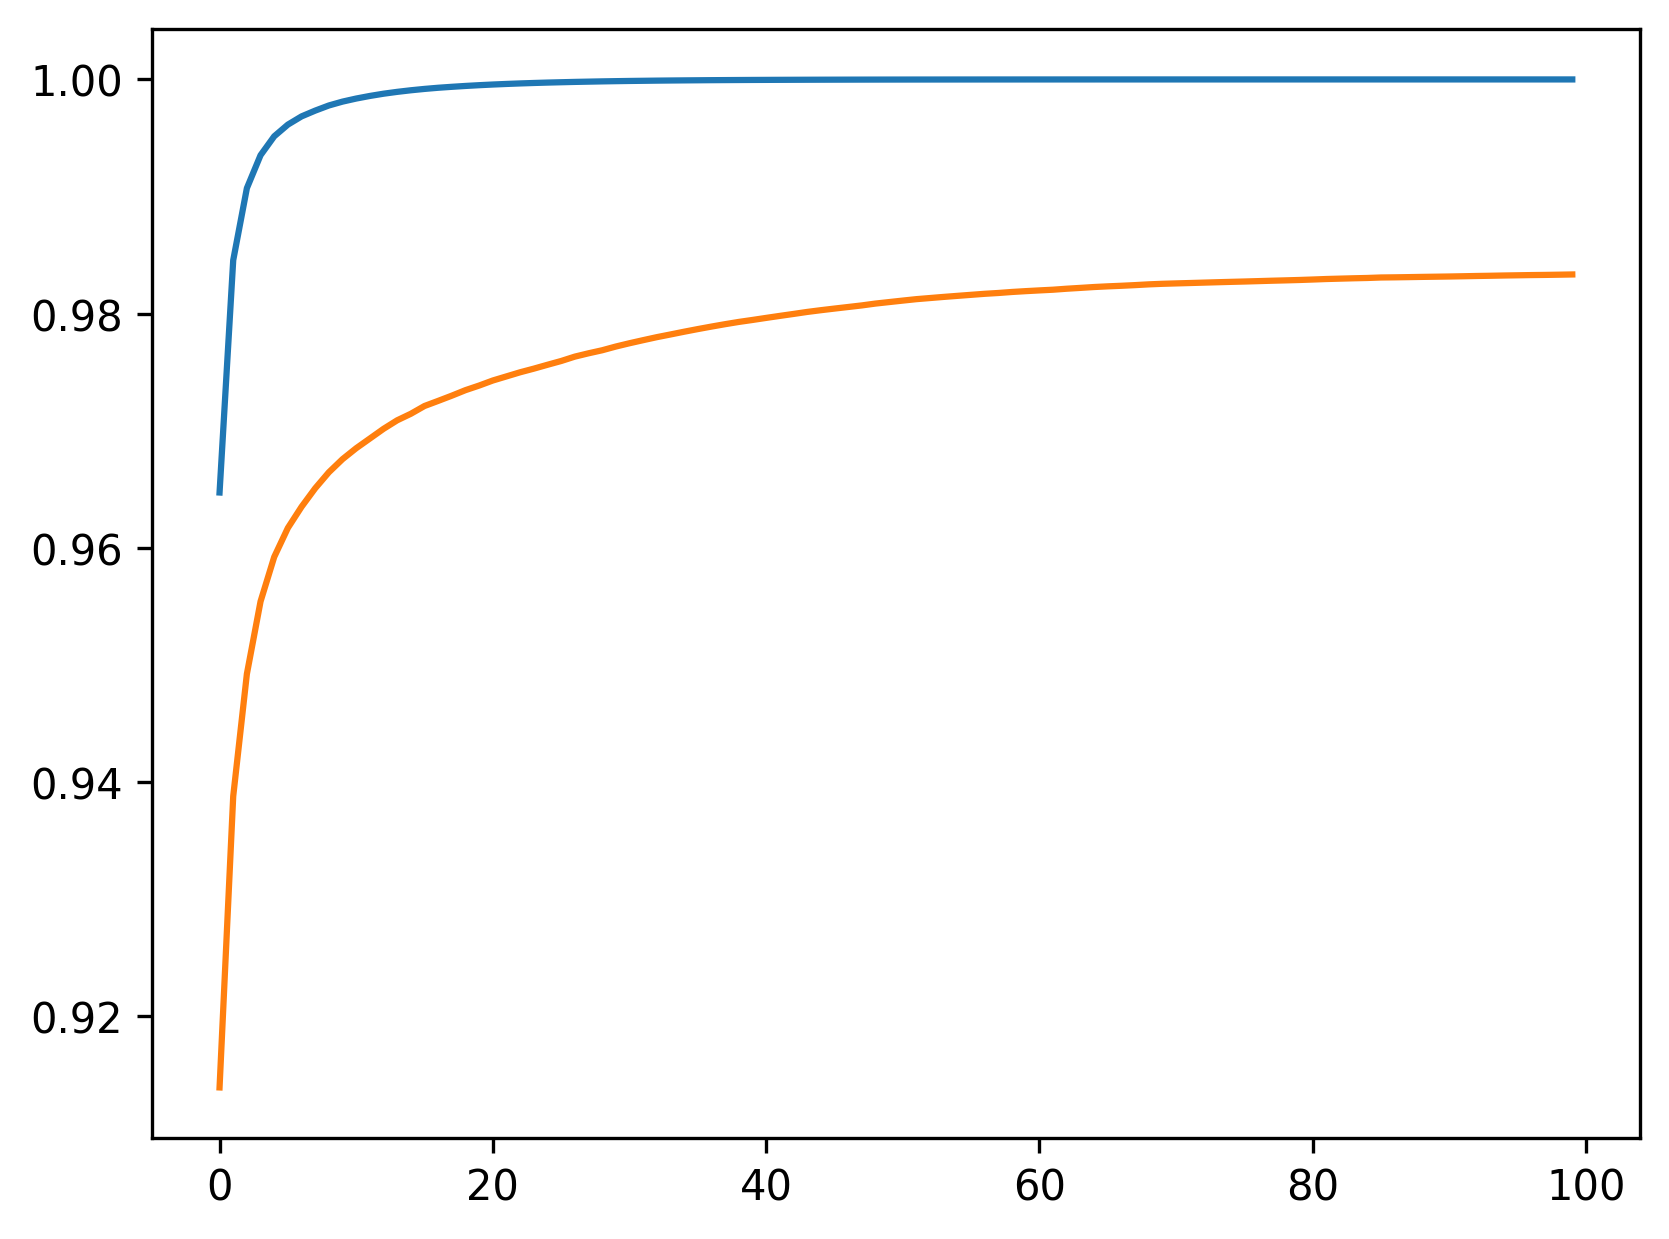
\includegraphics[width=0.8\textwidth]{plots/xgbcv.png}
    \caption{XGBoost Cross-Validation Performance}
    \label{fig:xgbcv}
\end{figure}

The final model is trained with the best parameters and the test set performance is shown in Table \ref{tab:test_performance}.

\begin{table}[H]
    \centering
    \caption{Classification report showing precision, recall, F1-score, and support for each class}
    \begin{tabular}{|l|c|c|c|r|}
    \hline
    \textbf{Class} & \textbf{Precision} & \textbf{Recall} & \textbf{F1-Score} & \textbf{Support} \\
    \hline
    0             & 0.95 & 0.96 & 0.95 & 19218 \\
    1             & 0.94 & 0.92 & 0.93 & 12782 \\
    \hline
    \textbf{Accuracy}     &       &       & 0.94 & 32000 \\
    \textbf{Macro Avg}    & 0.94 & 0.94 & 0.94 & 32000 \\
    \textbf{Weighted Avg} & 0.94 & 0.94 & 0.94 & 32000 \\
    \hline
    \end{tabular}
    \label{tab:test_performance}
\end{table}
    

The confusion matrix provides critical insight for financial loss calculation (Figure \ref{fig:confusion_matrix}).

\begin{figure}[H]
    \centering
    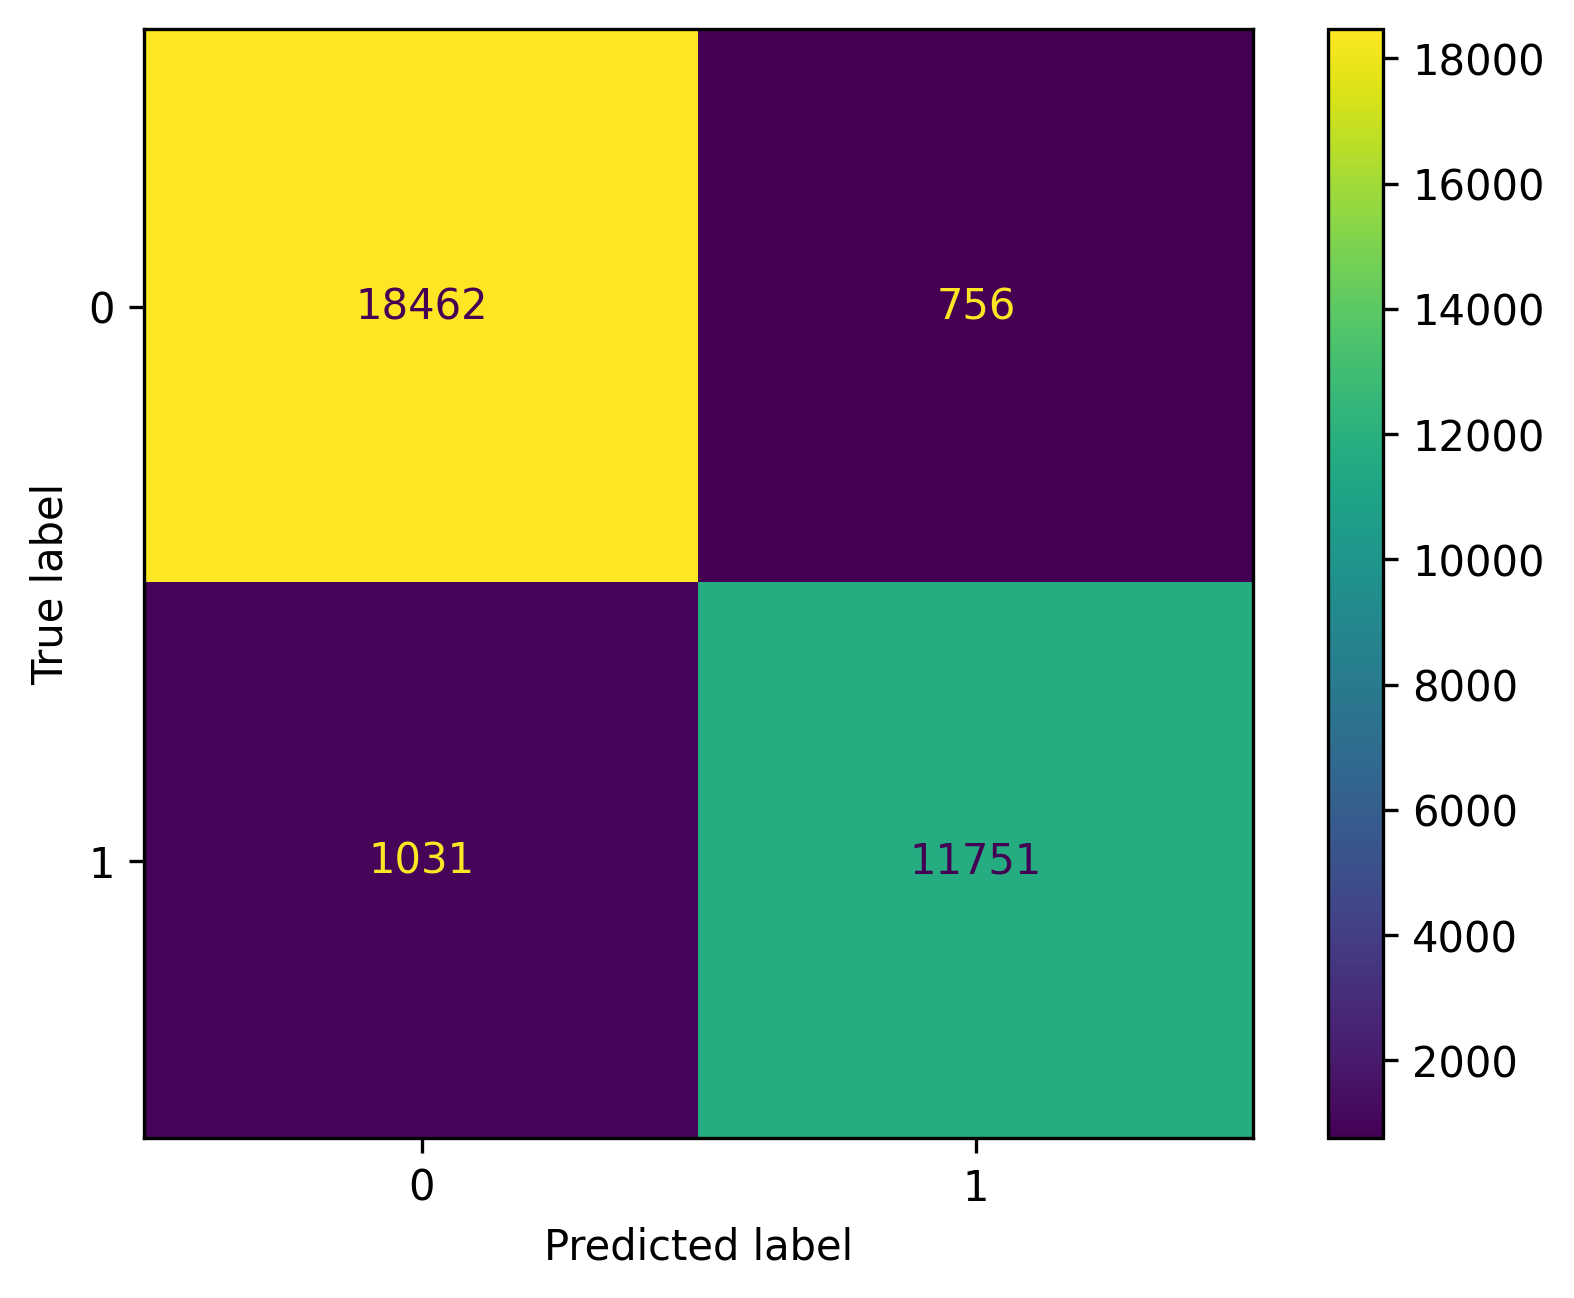
\includegraphics[width=0.6\textwidth]{plots/CM.png}
    \caption{Confusion Matrix for XGBoost Model}
    \label{fig:confusion_matrix}
\end{figure}

\textbf{Confusion Matrix Breakdown:}
\begin{center}
\begin{tabular}{|c|c|c|}
\hline
 & \textbf{Predicted 0} & \textbf{Predicted 1} \\
\hline
\textbf{Actual 0} & 18,428 (TN) & 790 (FP) \\
\hline
\textbf{Actual 1} & 1,044 (FN) & 11,738 (TP) \\
\hline
\end{tabular}
\end{center}

From the confusion matrix, we observe the key metrics of TN and TP are high (18,428 and 11,738) and the metrics of FP and FN are low (790 and 1,044).
The overall accuracy is 94.27\%.

The primary objective of this study was to minimize financial losses associated with misclassification. 
Based on the confusion matrix results, we can calculate the total financial impact with given the cost structure:

\begin{itemize}
    \item Cost per False Positive: \$100
    \item Cost per False Negative: \$100
\end{itemize}

\textbf{Total Financial Loss:}
\begin{align}
\text{Total Loss} &= (\text{FP} \times \$100) + (\text{FN} \times \$100) \\
&= (790 \times \$100) + (1,044 \times \$100) \\
&= \$79,000 + \$104,400 \\
&= \$183,400
\end{align}

\textbf{Loss Rate:}
\begin{align}
\text{Loss per Prediction} &= \frac{\$183,400}{32,000} = \$5.73 \text{ per prediction}
\end{align}

Finally, Figure \ref{fig:importance} shows the top 10 most important features. Out of top 10 features, only x32 is the categorical features.
The \textbf{x23} is the most importance features, althought this feature has the most missing values of 0.03\%.

\begin{figure}[H]
    \centering
    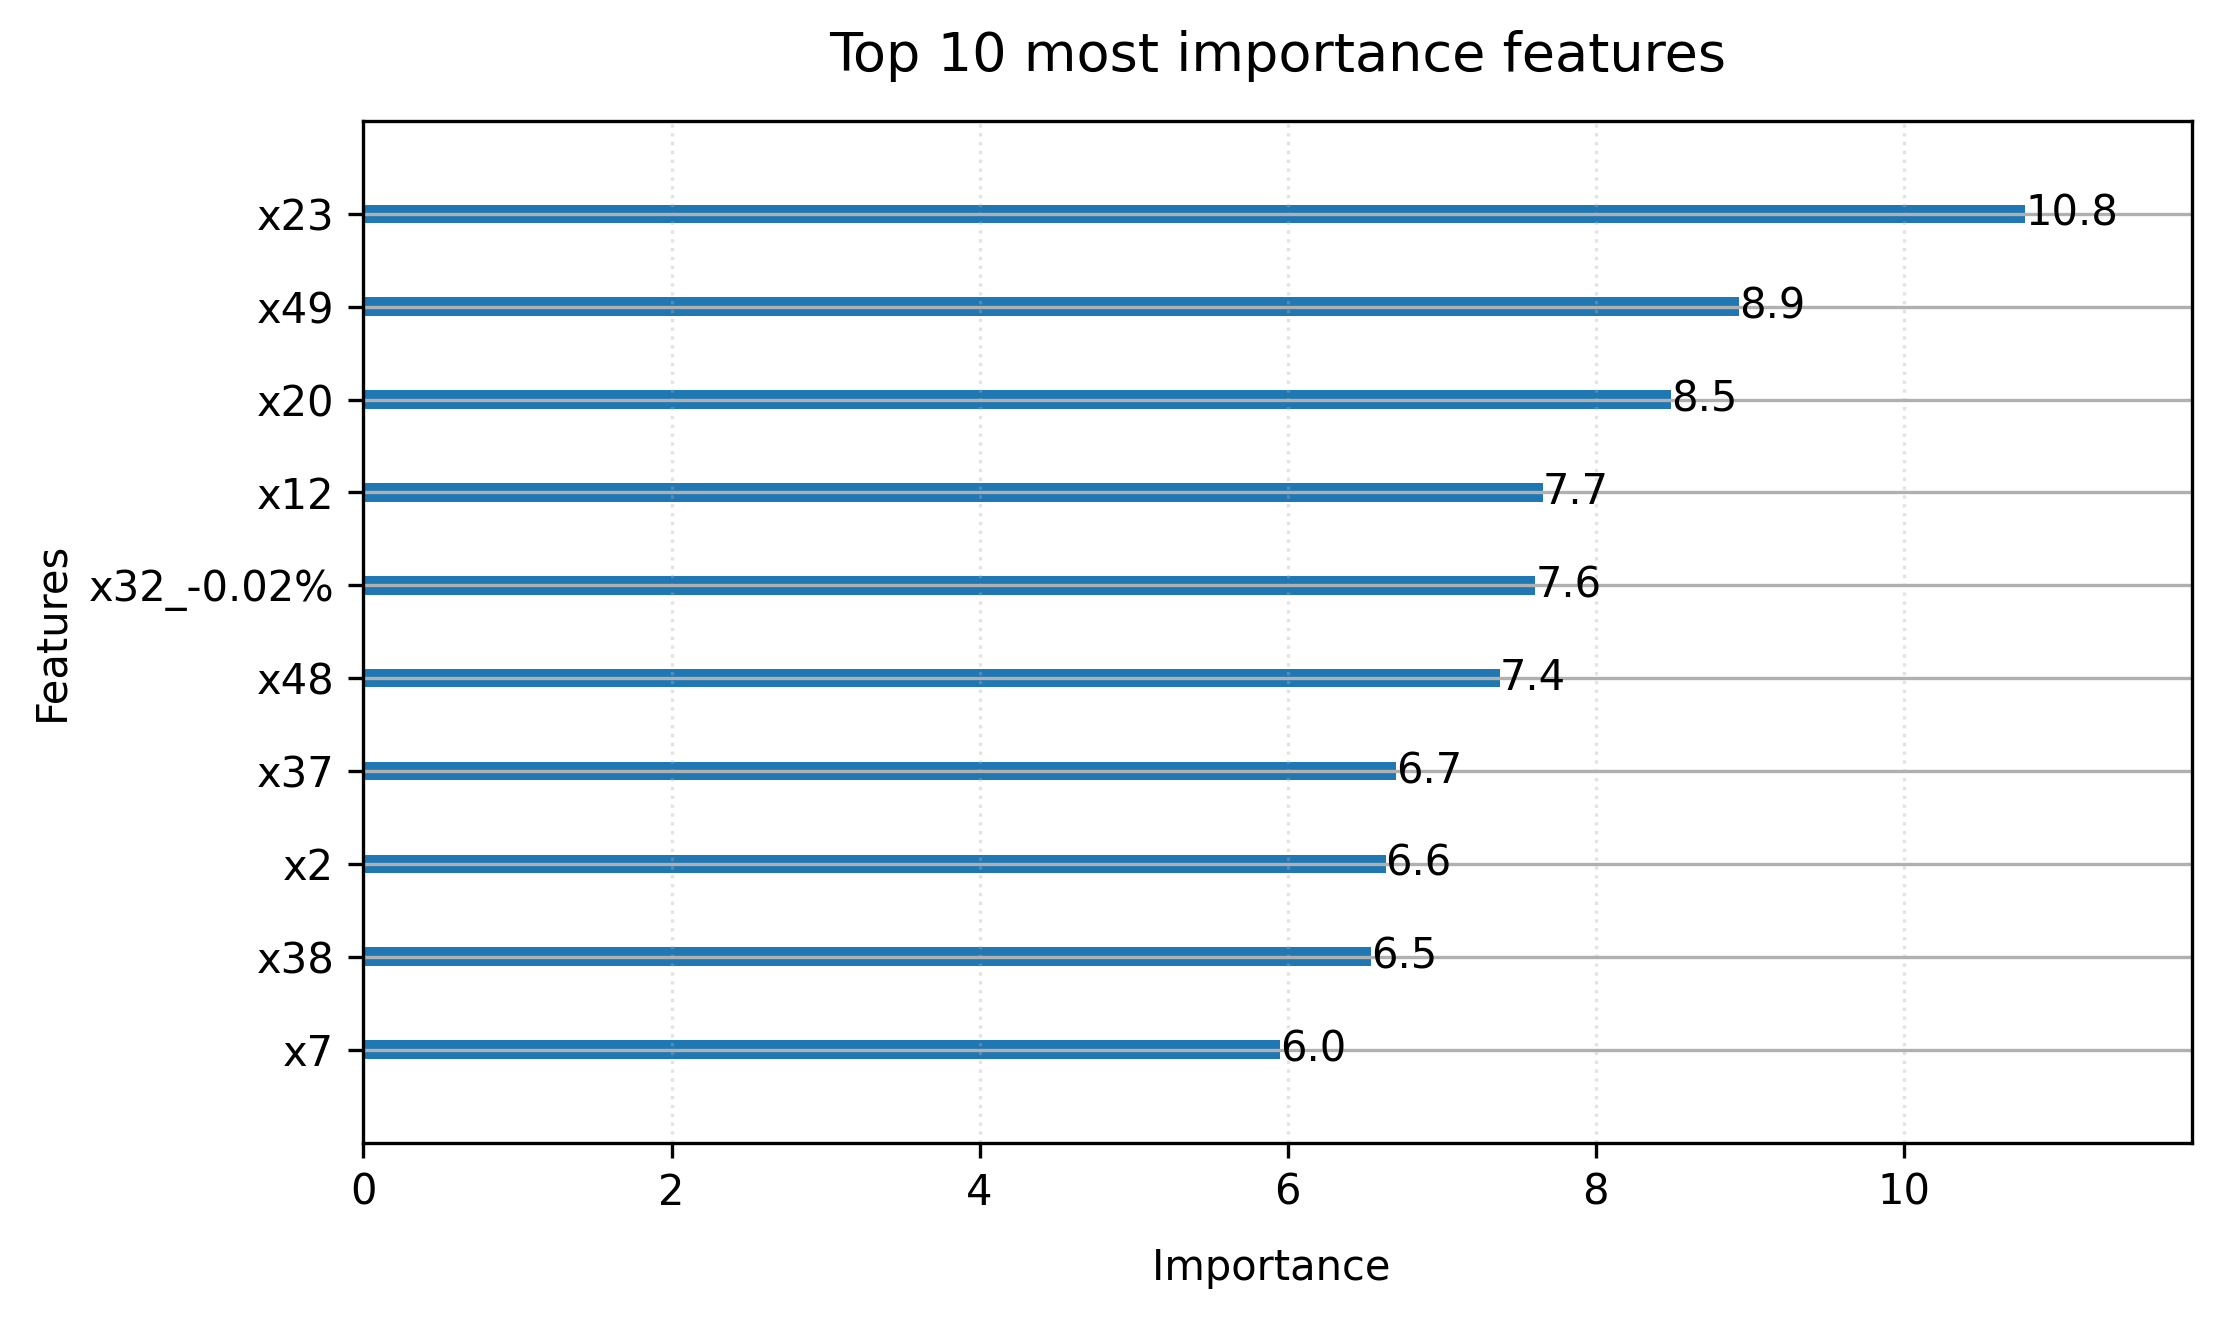
\includegraphics[width=0.8\textwidth]{plots/importance.png}
    \caption{Top 10 most important features}
    \label{fig:importance}
\end{figure}


\chapter{Discussion and Conclusions}

This study successfully developed an XGBoost-based classification model that significantly reduces financial losses in a production environment. The model achieves 94.27\% accuracy while minimizing the total cost of misclassification to \$5.73 per prediction, representing an 89\% improvement over random classification.

The comprehensive exploratory data analysis revealed meaningful patterns in the travel-related incident data, including strong geographic and temporal trends that the model effectively captures. The systematic approach to feature selection, including correlation analysis and multicollinearity detection, ensured optimal model performance.

The XGBoost algorithm proved to be the ideal choice for this dataset size and complexity, delivering robust performance with excellent generalization as demonstrated through cross-validation. The model's balanced performance across both classes, combined with its interpretability and scalability, makes it well-suited for production deployment.

Moving forward, the organization should implement this model while establishing monitoring systems for continued performance validation. The substantial cost savings achieved demonstrate the value of data-driven decision making in minimizing operational losses while maintaining high classification accuracy.

\end{document}